% !TeX root = ../Book2.tex
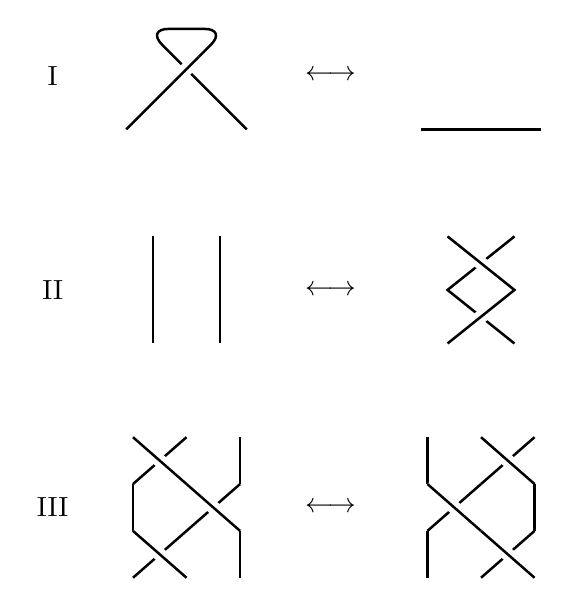
\begin{tikzpicture}[line width=.9pt,scale=.85,over/.style={preaction={draw=white,line width=4.8pt}}]
	\node at (-2.0,0.2) {I};
	\draw[rounded corners=8pt] (-.9,-.6)--(.6,.9)--(-.6,.9)--(.9,-.6);
	\draw[over] (-.18,.12)--(.18,.48);
	\node at (2.15,.2) {\(\longleftrightarrow\)};
	\draw (3.5,-.6)--(5.3,-.6);
	\begin{scope}[yshift=-2.2cm]
		\node at (-2.0,-.8) {II};
		\draw (-.5,0)--(-.5,-1.6);
		\draw (.5,0)--(.5,-1.6);
		\node at (2.15,-.8) {\(\longleftrightarrow\)};
		\draw (4.9,0)--(3.9,-.8)--(4.9,-1.6);
		\draw[over] (3.9,0)--(4.9,-.8)--(3.9,-1.6);
	\end{scope}
	\begin{scope}[yshift=-5.2cm]
		\node at (-2.0,-1.05) {III};
		\draw (0,0)--(-.8,-.7);
		\draw[over] (-.8,0)--(0,-.7);
		\draw (.8,0)--(.8,-.7);
		\draw (.8,-.7)--(0,-1.4);
		\draw[over] (0,-.7)--(.8,-1.4);
		\draw (-.8,-.7)--(-.8,-1.4);
		\draw (0,-1.4)--(-.8,-2.1);
		\draw[over] (-.8,-1.4)--(0,-2.1);
		\draw (.8,-1.4)--(.8,-2.1);
		\node at (2.15,-1.05) {\(\longleftrightarrow\)};
		\begin{scope}[xshift=4.4cm]
			\draw (.8,0)--(0,-.7);
			\draw[over] (0,0)--(.8,-.7);
			\draw (-.8,0)--(-.8,-.7);
			\draw (0,-.7)--(-.8,-1.4);
			\draw[over] (-.8,-.7)--(0,-1.4);
			\draw (.8,-.7)--(.8,-1.4);
			\draw (.8,-1.4)--(0,-2.1);
			\draw[over] (0,-1.4)--(.8,-2.1);
			\draw (-.8,-1.4)--(-.8,-2.1);
		\end{scope}
	\end{scope}
\end{tikzpicture}
